\documentclass{amsart}

\usepackage{tikz}

\begin{document}
	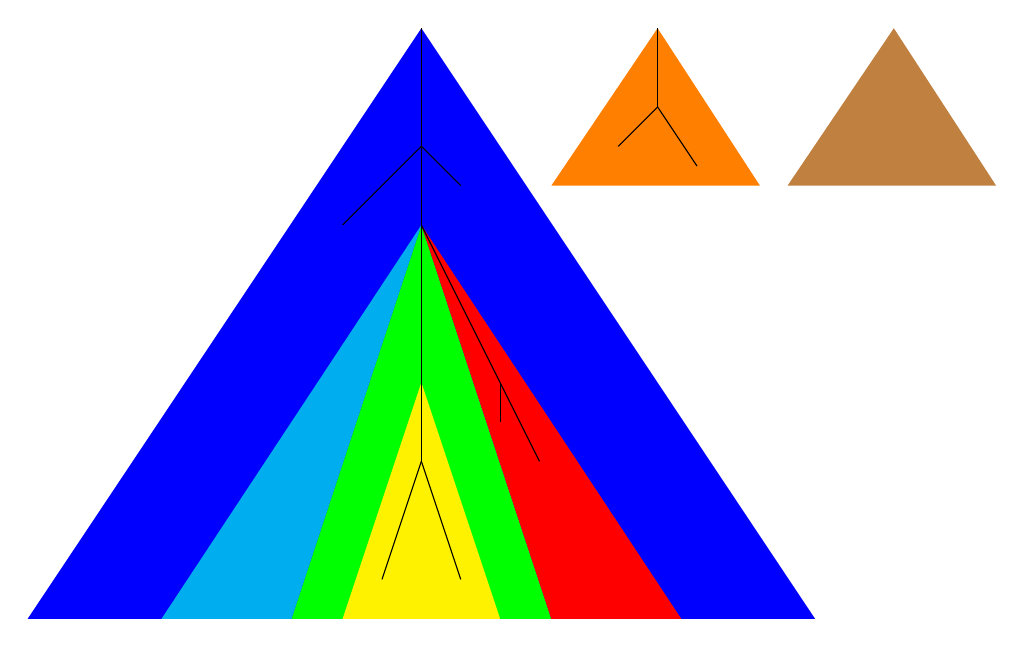
\begin{tikzpicture}[scale=.5]
		\path [fill=blue] (-10,-15) -- (0,0) -- (10,-15);
		\path [fill=orange] (3.3,-4) -- (6,0) -- (8.6,-4);
		\path [fill=brown] (9.3,-4) -- (12,0) -- (14.6,-4);
		
		\path [fill=green] (-3.3,-15) -- (0,-5) -- (3.3, -15);
		\path [fill=red] (3.3,-15) -- (0,-5) -- (6.6,-15);
		\path [fill=cyan] (-3.3,-15) -- (0,-5) -- (-6.6,-15);
		\path [fill=yellow] (0,-9) --  (-2,-15) -- (2, -15);

		%\draw [gray] (0,0) -- (-10,-15);
		%\draw [gray] (0,0) -- (10, -15);

		%\draw [gray] (0,-5) -- (-6.6,-15);
		%\draw [gray] (0,-5) -- (6.6, -15);

		%\draw [gray] (0,-5) -- (-3.3,-15);
		%\draw [gray] (0,-5) -- (3.3, -15);

		%\draw [gray] (0,-9) -- (-2,-15);
		%\draw [gray] (0,-9) -- (2, -15);
		
		
		\draw (0,0) -- (0,-3) node{};
		\draw (0,-3) --(1,-4) node{};
		\draw (0,-3) --(-2,-5) node{};
		
		\draw (0,0) --(0,-5) node{};

		\draw (0,-5) --(0,-9) node{};
		
		\draw (0,-9) --(0,-11) node{};
		\draw (0,-11) --(-1,-14) node{};
		\draw (0,-11) --(1,-14) node{};

		\draw (0,-5) --(2,-9) node{};
		\draw (2,-9) --(2,-10) node{};
		\draw (2,-9) --(3,-11) node{};
		
		
		\draw (6,0) -- (6,-2) node{};
		\draw (6,-2) --(7,-3.5) node{};
		\draw (6,-2) --(5,-3) node{};
	\end{tikzpicture}
	
	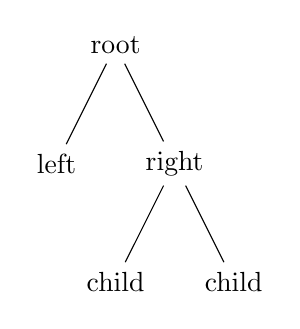
\begin{tikzpicture}
		\node {root}
			child {node {left}}
			child {node {right}
			child {node {child}}
			child {node {child}}
			};
	\end{tikzpicture}
\end{document}